\chapter{Implementation}
\label{ch:implementation}
\acresetall

This chapter goes into depth on how the design from the previous chapter is
implemented into the BATMAN protocol. Some code snippets will be shown in the
following sections when applicable, and the full source code can be found in
Appendix \ref{appendix:source}.

%\begin{figure}[h]
%	\centering
%	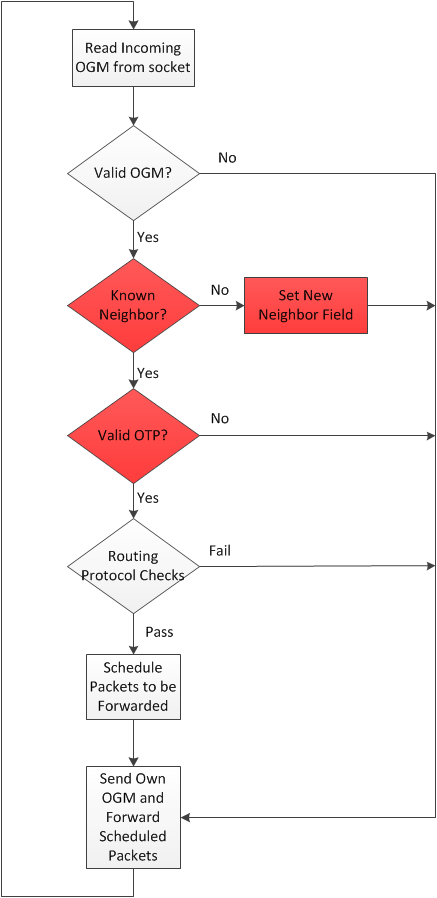
\includegraphics[totalheight=1\textheight]{images/batman_if_statements.png}
%	\caption{IF-Statements in the Batman Class}
%	\label{fig:batman_if_statements}
%\end{figure}

\section{OpenSSL Library}
All of the cryptographic functions such as encryptions, signatures, and X.509
public key certificate creation and verification are created using functions
from the OpenSSL library \cite{viega2002network}. This library was not in the
original implementation of BATMAN, and has to be installed on the computers running this modified version
and added to the Makefile for the BATMAN implementation. How to install the
correct OpenSSL library in a debian environment is explained in Appendix
\ref{appendix:lab_setup}, and the modified Makefile is part of the full source
code linked to in Appendix \ref{appendix:source}.

\section{Authentication Module}
Almost all functionality added to BATMAN is within the borders of a separate
class called \ac{AM}. The first thing to notice about the \ac{AM} is that it
runs in its own thread and sockets, so all authentication mechanisms run
concurrent to regular BATMAN routing operations. This separation was necessary
in order to have BATMAN behave normally during e.g. the authentication of a
node, so a large network should not suffer if an important node (centrally
located) is 'hung up' in e.g. authenticating another node.

\subsection{AM Thread}
In the setup phase in the original batman class, an \ac{AM} initiation function
called \texttt{am\_thread\_init} from the \ac{AM} class is called. This
function takes the network interface name and its corresponding IP address and broadcast
address as input. These values are then stored locally in in the AM class for
socket setup. For socket setup see Section \ref{subsect:am_socks}.

The function then goes on to create a new thread for the AM module which is the
main thread taking care of most of the additions in this implementation. The
thread first sets up two sockets for sending and receiving AM messages such as
handshakes and keystream-materials.

Next it generates a highly random (high entropy) master key using the OpenSSL
function \texttt{RAND\_bytes}, which has been properly seeded - see Section
\ref{subsect:posix.c}. This and an IV generated with OpenSSL's
\texttt{RAND\_pseudo\_bytes} is then used to generate a master key encryption
context for AES encryption, before deleting the master key. With the encryption
context the necessary internal memory used by OpenSSL for encrypting with this
key is stored, and therefore the key and IV is of no more use by themselves -
making it a sound security choice to delete the key (and IV) entirely.

The next important action is to generate either a \ac{PC0} or a \ac{PC} request
depending on whether you are a \ac{SP} or just a regular node trying to
authenticate with the network.

After these steps the ``initiation phase'' of the AM thread is complete, and the
rest of the code runs in a loop until the BATMAN daemon is terminated.

\subsection{AM Sockets}\label{subsect:am_socks}
Two sockets are used for the AM module, one for sending and one for receiving AM
messages. Both sockets are bound to the interface device given by the AM
initiation function. The receive socket is then bound to a designated port
64305, regular BATMAN runs on port 4305, and the send socket is explicitly
allowed to send to broadcast addresses. Sockets needs to be explicitly set to be
allowed to send to broadcast addresses in UNIX systems, as a protection
mechanism. A code snippet of the sockets set up is shown in the appendix under
Section \ref{code:sockets}.

There are several practical reasons to choose UDP sockets over TCP sockets for
this implementation. First and foremost, this system sends authentication
handshake messages and keystream-material messages to nodes which has no route
in the routing tables. If a connection-oriented protocol would try this the
messages would be blocked on the kernel level and not sent. With an
connectionless protocol like UDP no mechanisms will block this message being
sent, it will just send the message not bothering whether the message is ever
received by the recipient.

Second, TCP was created with wired networks in mind, observing much less packet
loss. In \acp{MANET} the packet losses are much higher than in wired and fixed
infrastructure networks, and as nodes move around direct paths between nodes
change much more frequently. TCP is not suitable for such environments because
it will lead to a huge amount of re-sending of packets to ``non-existant''
neighbors and much memory wasted in connection states being kept for dead links.

\subsection{Main Operation of the AM Thread}
Most of the interesting operation in the AM class happens within a single loop
running throughout the lifetime of the BATMAN daemon. The program flow
throughout this loop is shown in Figure \ref{fig:am_main_loop}.

\begin{figure}[h!]
	\centering
	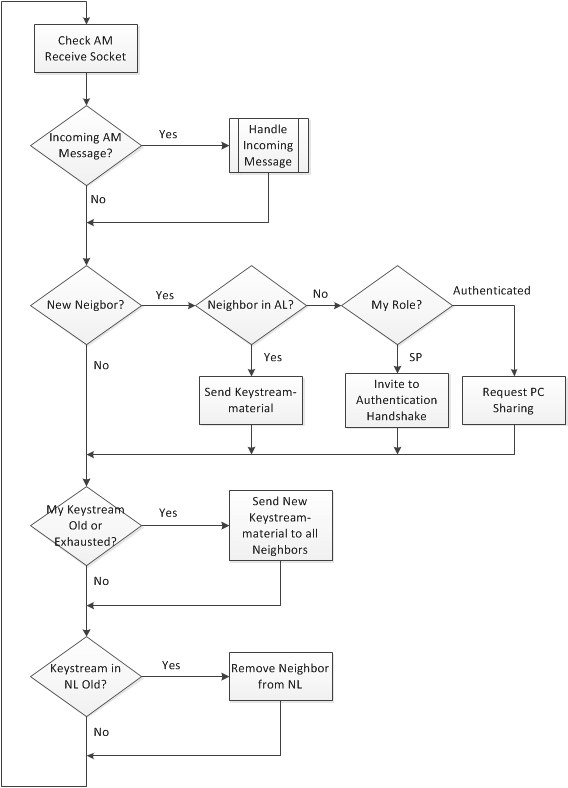
\includegraphics[width=\textwidth]{images/am_main_loop.png}
	\caption{Main program flow in AM class.}
	\label{fig:am_main_loop}
	\clearpage
\end{figure}

For clarity the figure leaves out certain details, but the most important
features are depicted. The handle incoming messages are shown as a sub-process
in the figure.  This is not true, but depicting all possible messages would not
fit the figure, and therefore left out altogether. However, each message are
described in the following sections.

The ``New Neighbor'' is one of the elements in the AM class that must be
triggered by the batman class. If the batman thread tells the AM thread a new
neighbor is discovered and the AM thread is in a ready state to handle new
neighbors the appropriate action is taken, whether the neighbor has been
authenticated with the network or not. Not shown in the figure is how a regular
authenticated node will act if a new neighbor which is not authenticated with
the network is handled, but this is taken care of in the batman class and not
here.

The two last parts should be self-explanatory, they simply check the current
time and then compares this against time values set on the nodes own current
keystream to check if its old, or if any keystreams from other neighbors in the
\ac{NL} are old and if so takes the appropriate action. Also checked is if a
nodes own keystream is getting exhausted, in which also the appropriate action,
namely creating and sharing a new one with each neighbor in the \ac{NL}.


\section{Proxy Certificates}
The \acp{PC} in this implementation are containers for short lived 1024 bits RSA
public keys used in a single session only. Most of the design choices were taken
into the implementation, but some however, were left due to time constraint.

One such was that the original proxy certificate X.509v3 extension, introduced
in RFC 3820 called ``proxyCertInfoExtension'' was not used to carry the policies as
intended. Most of the OpenSSL documentation is not released to the general
public for free, and this X.509v3 extension was no exception. The only examples
found, amongst the original proxy certificate implementations from the Globus
Project\footnote{Globus Project:
\url{http://www.globus.org/toolkit/downloads/}}, but using the exact same setup
did not work in my implementation. After some investigation it seems no open
source code projects using proxy certificates have been published for years,
giving me the idea that maybe the OpenSSL specifications have changed during
the last version updates and that proxy certificates have to be implemented
differently. The author have asked for an answer on this subject on both emails
to the developers of OpenSSL, the OpenSSL's mailinglists, and on an
OpenSSL ``IRC'' channel\footnote{OpenSSL IRC Channel: \#openssl on
\url{irc://irc.freenode.net}}.

As a replacement for this extension, a commonly used free-text extension called
\texttt{netscape\_comment} has been used and the policy has been written in
cleartext inside this comment. Because the design proposed used the
\texttt{id-ppl-anyLanguage} and allows the application to decide the language
the policy is written in, this should make no practical difference, other than
not being a strictly RFC 3820 proxyCertInfoExtension.

\subsection{Generating PC Requests}
As mentioned earlier the PC requests are generated prior to the main loop of the
AM thread. This means the request is generated and ready prior to discovering
new neighbors, so the authentication handshake can be performed as quick as
possible.

The request starts with creating and assigning a RSA key pair the size of 1024
bits. If the reader take a look into the implementation he or she will see that
the setup for an \ac{ECC} key pair is also there. Using ECC was only scrapped
at the very end because of problems regarding the keystream-material exchange
later on, where the author had problems with the ECIES algorithm.

The subject name is created a pseudo random function, contrary to using the
SHA-1 digest of the public key as proposed in the design. This was implemented
this way at the beginning quickly, and was supposed to be exchanged with the
message digest later on but because of time constraint there were no time to
test whether this subject name was set correctly. It should however be an easy
and relatively quick fix, but needs to be tested properly first - and probably
be encoded in Base64.

After this the proxy certificate extension is added using the following
function\\\texttt{openssl\_cert\_add\_ext\_req} as seen in Section
\ref{code:pc_ext}.

All this data is stored as a X.509\_REQ object and written to disk and sent
during the handshake in a PEM encoded format \cite{rfc1421}.

\subsection{Generating PCs}
Generating PCs are much the same as creating PC requests, with the addition of
signing the certificate, changing the subject name, setting the issuer name, and
setting the valid lifetime of the certificate. The issuer name is simply set to
the subject name of the \ac{SP} and the subject name is set as shown in Section
\ref{code:set_subject_name}. The valid lifetime is set from the current time,
and until 8 hours from creation.

\subsection{Verifying PCs}
In this implementation PCs and their public keys are not verified during the
initial authentication phase. This implementation use the physical locality as
the ``out-of-band verification'', which might be good enough if the SP only
use an ethernet cable which has to be directly connected to the new nodes trying
to authenticate themselves. However, in a real-world implementation this method
has to be revised!

However, when the initial authentication with the SP is complete, nodes do
verify each others' PCs by checking the signature against the SPs public key
using \texttt{X509\_verify} taking the received certificate and the SPs public
key as input.

\section{Authentication List}
When a node has verified another node, it stores some information about that
node within struct called \texttt{trusted\_node}. Then the struct is placed in a
list called \ac{AL} which stores one such struct for each known and trusted
node. Table \ref{tab:impl_al_content} shows how this data structure looks like:
\begin{table}[h]
	\centering
	\begin{tabular}{| l | l |}\hline
 		\textbf{Data type} & \textbf{Variable Name}\\\hline
		uint16\_t & id\\\hline
		uint32\_t & addr\\\hline
		uint8\_t & role\\\hline 
		unsigned char * & name\\\hline 
		EVP\_PKEY * & pub\_key\\\hline  
	\end{tabular}
	\caption{Trusted node struct of the AL.}
	\label{tab:impl_al_content}
\end{table}
At the beginning of the project, the AL was intended to be sent on the network
and was therefore made as an array, instead of a linked list. With additional
time this list should however be converted to a linked list for better
performance and less memory waste. The complete code snippet showing how a newly
verified node is added to the AL is shown in Section \ref{code:add_to_al}.

\section{Neighbor List}
Similarly when a node receives a new keystream-material message from a neighbor
the neighbor is added to the \ac{NL}. This list is also an array, and should
also be changed to a linked list, which contains a data structure called
\texttt{trusted\_neigh}. Below Table \ref{tab:impl_nl_content} shows this new
data structure:
\begin{table}[h]
	\centering
	\begin{tabular}{| l | l |}\hline
 		\textbf{Data type} & \textbf{Variable Name}\\\hline
		uint16\_t & id\\\hline
		uint32\_t & addr\\\hline
		uint64\_t & window\\\hline 
		uint16\_t & last\_seq\_num\\\hline
		unsigned char * & mac\\\hline 
		time\_t & last\_rcvd\_time\\\hline
		uint8\_t & num\_keystream\_fails\\\hline 
	\end{tabular}
	\caption{Trusted neighbor struct of the NL.}
	\label{tab:impl_nl_content}
\end{table}
Note here that while the design and implementation changed during this thesis
things have changed, and what used to be a \ac{MAC} in the NL is now a
keystream, but the names have not been changed in the current version of the
implementation.

The code snippet in Section \ref{code:add_to_nl} shows what happens whenever a
new neighbor is added, or a new keystream-material is received from a neighbor.
The code snippet in Section \ref{code:rem_from_nl} shows what happens whenever a
node is removed from the NL due to inactivity, i.e. not received its
keystream-material for 130 seconds.

\section{Keystream Generation}
Before a keystream can be generated, its keystream-material must be generated
(and sent). The IV and nonce are both generated using OpenSSL's
\texttt{RAND\_pseudo\_bytes} generating 16 and 767 Bytes of pseudo random data,
respectively. The generation of the ephemeral key is created using AES-CBC as
shown in the code snippet in Section \ref{code:gen_eph_key}.

When the keystream-material has been created, they can be used to create the
full keystream on both ends. First the original nonce is encrypted using the
ephemeral key and IV as inputs to OpenSSL's AES-CBC encryption. Next one tenth
(1/10) of the nonce will be XOR'ed with 1 and encrypted again with the AES-CBC
encryption, using the same key but using a part of the previous ciphertext as
IV. This is done 9 times, so the second round the second part (between 2/10 and
3/10) of the nonce will be XOR'ed with 2 and encrypted with the same key and IV
from previous ciphertext and so on until ten different (1 original and 9
modified) nonces has been encrypted. All the ciphertexts is then added to one
large buffer, which is this node's keystream. All of the operations above is
shown in the code snippet in Section \ref{code:gen_keystream}.

\section{Using One-Time Passwords}
\acp{OTP} are handled within the context of the original BATMAN protocol because
adding and verifying them is performed when the original protocol receives or
sends them. How to add the OTPs are described in Section
\ref{subsect:schedule.c} while how to verify them are described in Section
\ref{subsect:batman.c}.

\section{Changes to the BATMAN Protocol}
Some changes are BATMAN specific or needs to be called from within the original
BATMAN protocol and these changes are described here.

Figure \ref{fig:extended_ogm} shows how the modified batman packets, or
\acp{OGM}, look like. The white area is not changed, except an unused version
number is taken and used in the 'Version' field at the outset of the packet. The
red area is added by this implementation, containing both an \ac{OTP} and its
sequence number in the keystream.

\begin{figure}[h]
	\centering
  	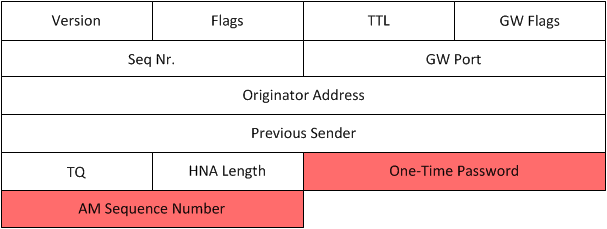
\includegraphics{images/extended_ogm.png}
  	\caption{Modified routing announcement (OGM) for extended BATMAN.}
	\label{fig:extended_ogm}
\end{figure}

\subsection{POSIX.C}\label{subsect:posix.c}
It is within the posix.c class that the daemon's main function that initialized
the whole program lies. In here a small but important modification was made.
Before allowing the daemon to start, OpenSSL's pseudo random number generator
(PRNG) has to be seeded with much high entropy random data. This is done by
taking 1024 bytes from the UNIX environment's \emph{/dev/urandom}. If this
seeding should fail, the daemon is not started and the program killed.

\subsection{BATMAN.C}\label{subsect:batman.c}
It is in this class where the main thread in the original BATMAN runs, where it
receives \acp{OGM}, decides how to handle them, and whether to schedule to send
own or re-broadcast other nodes' \acp{OGM}. Before entering the main loop, this
class has been modified to initiate the AM class by calling
\texttt{am\_thread\_init}.

Inside the main loop which is loops for each received \ac{OGM} there has been a
modification to verify the \ac{OTP} appended to the \ac{OGM}. If the
verification check is not passed, the \ac{OGM} is dropped, and possibly the AM
class is told there is a new node. The interesting code snippet from this class
can be found in Section \ref{code:ext_batman} in it entirety.

TODO: NEW FIGURE SHOWING THE BATMAN FLOW CHART HERE!

Figure XXXX shows the flow chart through the main loop in BATMAN. Here you can
see where the AM modifications are put, and hopefully understand why they are
put there. The first checks before the modification are almost like sanity
checks, which must be passed before testing the \acp{OTP} should even be
considered. After the AM extension there are many checks which are more specific
to the routing algorithm, but they do not affect whether the \acp{OTP} should be
checked, and if the OGM is received from a new neighbor the AM extension has to
notify the AM class of a new neighbor before allowing the the subsequent checks
to be made, or the OGM will be handled when it quite possibly should not.

\subsection{SCHEDULE.C}\label{subsect:schedule.c}
In the schedule class there are two functions which needs to be modified. The
two functions \texttt{schedule\_forward\_packet} and
\texttt{schedule\_own\_packet} generates and puts \acp{OGM} in a queue waiting
to be send on behalf of other nodes or itself, respectively. The modifications
are the same using only different available parameters, and is shown in Section
\ref{code:ext_schedule}.

Again there is some variable name discrepancy because the design and
implementation has evolved during the work of this thesis. The \texttt{auth}
variable name used actually means \ac{OTP} and the \texttt{auth\_value} means
the whole keystream. The line below means that a value of 2 bytes size is to
be copied from the keystream to the OTP value in the bat\_packet, or OGM.\\
\texttt{memcpy(bat\_packet-$>$auth, auth\_value+2*auth\_seq\_num, 2);}.
